% Interpretetabiliyt vs error and how we approach the high accuracy models






GPSR offers the advantage of generating a population of equations, providing users with the flexibility to choose the equation that best suits their specific needs. Typically, the optimal equation strikes a balance between simplicity and accuracy. However, certain scenarios may necessitate either maximum accuracy or very simple equations. This study presents various models with varying levels of accuracy and complexity. The SIF equation was derived using two methods from the $f_w$, $m$, and $g$ equations. The first method involved using fixed $f_w$ and $m$ equations, as the $g$ equation has the most significant impact on overall SIF accuracy. The equations obtained through this method are illustrated in Figure \ref{fig:perato_front}. The second method employed every possible combination of the $f_w$, $m$, and $g$ equations generated by Bingo, with the extracted equations depicted in Figure \ref{fig:perato_front_everything}. To facilitate comparison with the Raju and Newman equation, models were selected based on similar errors and complexities, as shown in Figure \ref{fig:perato_front_everything_ant_more}. The comparison revealed that Bingo outperforms the Raju and Newman equation in both complexity and error. Models with similar complexity demonstrated lower errors, while models with similar errors exhibited considerably lower complexities.

When applying the same approach as Raju and Newman to decompose $K$ using $f_w$, $M$, and $g$, the influence of $c/b$ is not entirely captured. The finite width of the model is considered only in the function $f_w$, which is not dependent on $\phi$. Consequently, there is no coupling between $\phi$ and $c/b$. This is evident in Figure \ref{fig:perato_front_everything}, where models allowing $c/b$ in $g$ outperform those that do not, particularly beyond a complexity of approximately 40. This discrepancy is observed specifically in models derived from every combination of $f_w$, $M$, and $g$. However, in the case of fixed $f_w$ and $M$ functions, whether or not $c/b$ is utilized in $g$ does not seem to alter the results, as shown in Figure \ref{fig:perato_front}. This is attributed to the specific $f_w$ equation chosen not being influenced by $c/b$ in $g$. Neglecting the interaction between $\phi$ and $c/b$ allows for the rapid creation of simpler models, significantly reducing the number of FE models required for training. Nonetheless, if a highly accurate model is essential, employing the entire domain for training enables the attainment of higher accuracy.



\subsection{Model limitations}

It was observed that, across all trained Bingo models, the highest errors occurred at the crack surface where $\phi$ is close to $0$ or $\pi$ and when $a/c$ is at its smallest value of $0.2$. At the crack surface where $\phi = \pi, 0$, the SIF values exhibit a sharp decline due to the influence of plane stress vs. plane strain conditions. The Bingo model struggles to fully capture this region because of a lack of data at the surfaces. It might be possible to address these surface effects by introducing an additional correction factor that specifically accounts for the model's surfaces. The reason for the highest errors occurring at $a/c = 0.2$ is that this represents the lower bound of the training data, and there is also a significant change in the SIF data in this region. Without information about SIFs for values smaller than $a/c = 0.2$ in the training data, Bingo fits this region of the data less accurately. Including smaller aspect ratios in the training data could likely reduce the maximum error of the model. However, it's worth noting that $a/c = 0.2$ is already a relatively small aspect ratio, and the rest of the domain with aspect ratios above $a/c = 0.2$ have very low error.


\subsection{Comparison with Black Box methods}



Comparing the results shown here from Bingo with other ML methods such as the ones used in \cite{Tushar}. Figure \ref{fig:bingo_ml_comp} shows Bingo and the Raju-Newman equation compared with two commonly used ML methods for a data-set of this size, support vector machine regression (SVM) and random forest regression (RFR). Using the optimal hyper-parameters from \cite{Tushar} and training directly on $K$ results in the square markers on the plot. Training the models again using the mechanics bases approach used in this research, results in the circle points. From this figure, the error of the RFR is reduced by using the mechanics based approach, while the SVM produces worse error when using the mechanics based approach. One possible reason that the SVM produces a worse model when using the mechanics based approach, is that it cannot fit to the smaller data-sets, while Bingo and RFR are easily able to fit to fewer data-points. It is shown in \cite{tushar} that as the data-points decrease to 100 that SVM performs worse. Being able to produce accurate models with fewer data-points is a strength as having many training examples is rarely feasible. Comparing the evaluation times of each of the ML models shown in \ref{fig:bingo_ml_comp} shows that bingo and the Raju-Newman have similar evaluation times, however, the black box models are slower with the random forest taking 3 seconds to evaluate the data-set, and SVM taking 40 seconds. 
\begin{figure}
    \centering
    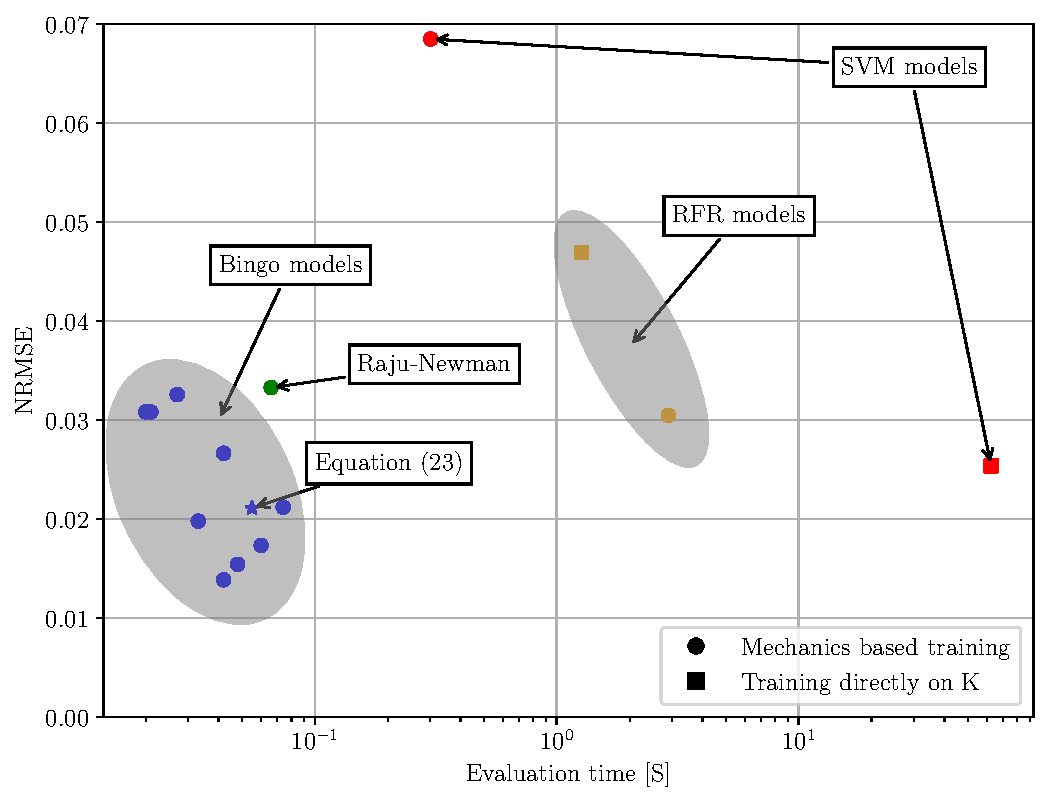
\includegraphics[width=\textwidth]{Figures_pdf/bingo_ml_comp.pdf}
    \label{fig:bingo_ml_comp}
    \caption{Plot comparing training times and errors between Bingo, Raju-Newman equation, RFR, and SVM. The circular markers were all trained using the mechanics based approach presented in this research, the square makers were trained directly on K. The evaluation times were measured on one core of an Intel i7-4790 with 32Gb DDR3 RAM at 1600 MHz on a data-set containing 150k data-points.}
\end{figure}
 

Bingo outperforms SVM and RFR both in evaluation time and error, while also producing an explainable closed form equation. Some of the Bingo models only needed a small subset of the data to be able to predict SIF for the entire domain. Bingo does, however, have a downside in its long training time on the order of hours to days, while SVM and RFR can be trained very quickly on the order of seconds to minutes. Bingo takes more effort than SVM and RFR to create a model for this data-set, however, the final model created by Bingo outperforms SVM, RFR, and the Raju-Newman equation in all metrics. 





